
\documentclass[12pt]{article}
\usepackage{geometry}
\geometry{a4paper}


\usepackage{color}
\usepackage{hyperref}
\usepackage{amsmath}
\usepackage{amsfonts}
\usepackage{amssymb}
\usepackage{graphicx}
\usepackage{tcolorbox}
\usepackage{listings}
\usepackage{here}
\usepackage{txfonts}
\usepackage{algorithm}
\usepackage{algorithmic}
\usepackage{siunitx}
\usepackage{xcolor}
\usepackage{ascmac}
%\usepackage{fancybx}

\lstset {language = c++,
  basicstyle = \ttfamily \scriptsize,
  commentstyle = \textit,
  frame = tRBl,
  framesep = 5pt,
  showstringspaces = false,
  numbers = left,
  stepnumber = 1,
  numberstyle = \tiny,
  tabsize = 2,
  keywordstyle = \bfseries \color{blue},
  stringstyle=\color{magenta},
  commentstyle=\color{red},
  morecomment=[l][\color{red}]{\#}
  showstringspaces=false, % don't mark spaces in strings
}
\newcommand{\bi}[1]{\mathbf{#1}}
\newcommand{\bs}[1]{\boldsymbol{#1}}  % bold for greek characters
\newcommand{\bbR}{\mathbb{R}}

\author{Nobuyuki Umetani}


\title{Finite Element Method:\\ Linear Elastic Material \footnote{This is a memorandum to write down what the forgetful author studied a long time ago. Surely it contains many mistakes. Excuse me. It is appreciated if you let me know if you have any comments or suggestions. }}
\author{Nobuyuki Umetani}


\begin{document}
\maketitle
\tableofcontents

\begin{figure}[hpbt]
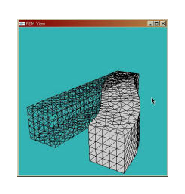
\includegraphics[width=5cm]{images/linear_solid3d.eps}
\end{figure}


\section{linear elastic body}

\subsection{Distortion in Linear Elastic Body}


For linear elastic bodies, the linear distortion $\epsilon$ is expressed as follows.

\begin{equation}
\bi{\epsilon}=\frac{1}{2}(\nabla_X\otimes\bi{u}+\bi{u}\otimes\nabla_X)
\end{equation}

\begin{equation}
\epsilon_{ij}=\frac{1}{2}(\frac{\partial u_i}{\partial X_j}+\frac{\partial u_j}{\partial X_i})
\end{equation}


Here $\bi{u}$ is the displacement from the non-deformed state.


\subsection{Constitutive expression of linear elastic body}


The stress $\bi{\sigma}$ of an isotropic linear elastic body can be written based on linear strain as follows.

\begin{equation}
\bi{\sigma}=\lambda({\rm tr}\bi{\epsilon})\bi{I}+2\mu\bi{\epsilon}
\end{equation}


However, $\lambda$ and $\mu$ are constants of $Rame$.
Write this as a component and it is as follows,

\begin{equation}
\sigma_{ij}=\lambda\epsilon_{kk}\delta_{ij}+2\mu\epsilon_{ij}
\end{equation}


Moreover, $\lambda$, $\mu$ has the following relationship with Young's modulus $E$ and Poisson ratio $\nu$ as follows.

\begin{eqnarray}
\lambda &=& \frac{E\nu}{(1+\nu)(1-2\nu)}\\
\mu &=& \frac{E}{2(1+\nu)}
\end{eqnarray}


\subsection{Problem setting}


\begin{figure}[hpbt]
\center
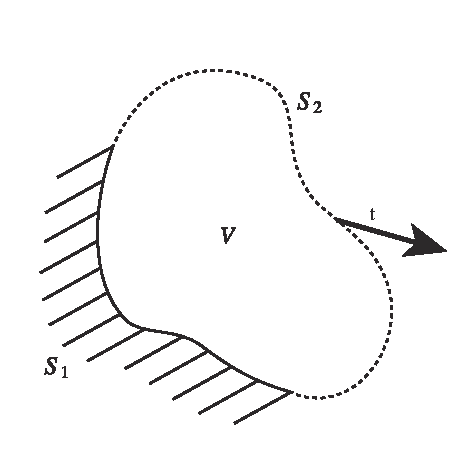
\includegraphics[width=80mm]{images/solid_domain}
\end{figure}

Displacement is fixed on $S_1$.

\begin{equation}
u=\bar{u} \quad ( \quad on \quad S1 \quad )
\end{equation}


Such boundary conditions are called fixed boundary conditions and displacement boundary conditions.

Stress is applied on $S_2$.

\begin{equation}
\bi{\sigma}^T\cdot\bi{n}=\bi{t} \quad ( \quad on \quad S2 \quad )
\end{equation}


Such a boundary condition is called a stress boundary condition.



\subsection{weak formalization}


Basically, the linear elastic body deforms the equilibrium equation to weak formalization, but we do numerical approximation there. When dealing with a large deformation, the original equilibrium equation is largely changed so that it shifts. However, it is less affected by minute deformation.

From Cauchy's first principle

\begin{equation}
\rho\left.\frac{\partial v}{\partial t}\right|_X=\rho\bi{g}+\nabla\cdot\bi{\sigma}
\end{equation}


An object in a static equilibrium state satisfies the following expression because the acceleration is 0

\begin{equation}
-\nabla\cdot\bi{\sigma}=\rho\bi{g}
\end{equation}


To weakly formalize it, multiply both sides of arbitrary function $\delta u$ which becomes 0 on $S_1$ and integrate it with $V$ before deformation.

\begin{equation}
-\int_V\delta u\cdot(\nabla\cdot\bi{\sigma})dV=\int_V\delta u\cdot\rho\bi{g}dV
\end{equation}


Modify the integrand of the first term on the left side


\begin{eqnarray}
\delta u\cdot(\nabla\cdot\bi{\sigma})
&=& \delta u_j\frac{\partial\sigma_{ij}}{\partial x_i}\simeq\delta u_j\frac{\partial\sigma_{ij}}{\partial X_i}\\
&=& \frac{\partial}{\partial X_i}(\delta u_j\sigma_{ij})-\frac{\partial\delta u_j}{\partial X_i}\sigma_{ij}\\
&=& \frac{\partial}{\partial X_i}(\delta u_j\sigma_{ij})-\frac{1}{2}(\frac{\partial\delta u_j}{\partial X_i}+\frac{\partial\delta u_i}{\partial X_j})\sigma_{ij}=\frac{\partial}{\partial X_i}(\delta u_j\sigma_{ij})-\delta\epsilon_{ij}\sigma_{ij}\\
&=& \nabla\cdot(\sigma\cdot\delta\bi{u})-\delta\bi{\epsilon}:\bi{\sigma}
\end{eqnarray}

Substituting this

\begin{equation}
 -\int_V\nabla\cdot(\sigma\cdot\delta\bi{u})-\delta\bi{\epsilon}:\bi{\sigma}dV=\int_V\delta u\cdot\rho\bi{g}dV
\end{equation}


Move the first term of the integrand on the left side to the right side

\begin{equation}
 \int_V\delta\bi{\epsilon}:\bi{\sigma}dV=\int_V\delta u\cdot\rho\bi{g}dV+\int_V\nabla\cdot(\sigma\cdot\delta\bi{u})dV
\end{equation}


Adapting Gauss' divergence theorem to the second term on the right side,

\begin{equation}
\int_V\bi{\sigma}:\delta\bi{\epsilon}dV=\int_V\delta u\cdot\rho\bi{g}dV+\int_{\partial V}N\cdot(\sigma\cdot\delta\bi{u})dS
\end{equation}


Modify the second term on the right side.

\begin{eqnarray}
\int_{\partial V}N\cdot(\sigma\cdot\delta\bi{u})dS
&=& \int_{S_2}N\cdot(\sigma\cdot\delta\bi{u})dS\\
&\simeq& \int_{S_2}\bi{n}\cdot(\sigma\cdot\delta\bi{u})dS\\
&=& \int_{S_2}\delta\bi{u}\cdot\sigma^T\cdot\bi{n}dS=\int_{S_2}\delta\bi{u}\cdot\bi{t}dS
\end{eqnarray}

When this is substituted, the weakly formatted problem eventually becomes as follows.


\begin {tcolorbox}[title=Weakly Formulated Governing Equation]
\begin{equation}
\left\{\begin{array}{l}\int_V\bi{\sigma}:\delta\bi{\epsilon}dV=\int_V\rho\delta\bi{u}\cdot\bi{g}dV+\int_{S_2}\delta\bi{u}\cdot\bi{t}dS\quad\{ \delta\bi{u} \mid \delta\bi{u}=0 \quad (on \quad S_1) \}\\ \bi{u}=\bar{\bi{u}}\qquad (\quad on \quad S_1 \quad)\end{array}\right.
\end{equation}
\end{tcolorbox}

\subsection{Transformation of Weakly Formulated Governing Equations to Display Using Displacement}


Although weak formalization was possible with the above equation, since we solve the displacement as a variable, we have to transform the above weak form equation into an expression with displacement.

Substituting constituent formulas of linear elastic bodies into stress,

\begin{equation}
\int_V(\lambda({\rm tr}\bi{\epsilon})\bi{I}+2\mu\bi{\epsilon}):\delta\bi{\epsilon}dV=\int_V\rho\delta\bi{u}\cdot\bi{g}dV+\int_{S_2}\delta\bi{u}\cdot\bi{t}dS
\end{equation}

\begin{equation}
\int_V \lambda({\rm tr}\bi{\epsilon})({\rm tr}\bi{\delta\epsilon})+2\mu\bi{\epsilon}:\delta\bi{\epsilon}dV=\int_V\rho\delta\bi{u}\cdot\bi{g}dV+\int_{S_2}\delta\bi{u}\cdot\bi{t}dS
\end{equation}

Applying the summary rule to $i$, $j$ and writing with components will be as follows.

\begin{equation}
\int_V \lambda\epsilon_{jj}\delta\epsilon_{ii}+2\mu\epsilon_{ij}\delta\epsilon_{ij}dV=\int_V\rho\delta u_i g_idV+\int_{S_2}\delta u_i t_idS
\end{equation}

\begin{equation}
\int_V \lambda\frac{\partial u_j}{\partial X_j}\frac{\partial \delta u_i}{\partial X_i}+2\mu\frac{1}{2}\left(\frac{\partial u_i}{\partial X_j}+\frac{\partial u_j}{\partial X_i}\right)\frac{1}{2}\left(\frac{\partial \delta u_i}{\partial X_j}+\frac{\partial \delta u_j}{\partial X_i}\right)dV=\int_V\rho\delta u_i g_idV+\int_{S_2}\delta u_i t_idS
\end{equation}


Expand the second term in the left-hand integrand
\begin{equation}
\int_V \lambda\frac{\partial u_j}{\partial X_j}\frac{\partial \delta u_i}{\partial X_i}+\frac{1}{2}\mu\left(\frac{\partial u_i}{\partial X_j}\frac{\partial \delta u_i}{\partial X_j} + \frac{\partial u_j}{\partial X_i}\frac{\partial \delta u_i}{\partial X_j} + \frac{\partial u_i}{\partial X_j}\frac{\partial \delta u_j}{\partial X_i} + \frac{\partial u_j}{\partial X_i}\frac{\partial \delta u_j}{\partial X_i}\right)dV=\int_V\rho\delta u_i g_idV+\int_{S_2}\delta u_i t_idS
\end{equation}

Subscript of $\delta u$ is changed to $i$ and suffix of $u$ becomes $j$ Subscript substitution is as follows

\begin{tcolorbox}[title=Governing equations weakly formulated based on displacement]
\begin{eqnarray}
\left\{\begin{array}{l}\int_V \lambda\frac{\partial u_j}{\partial X_j}\frac{\partial \delta u_i}{\partial X_i} + \mu\left(\frac{\partial u_j}{\partial X_k}\frac{\partial \delta u_i}{\partial X_k}\delta_{ij} + \frac{\partial u_j}{\partial X_i}\frac{\partial \delta u_i}{\partial X_j} \right)dV=\int_V\rho\delta u_i g_idV+\int_{S_2}\delta u_i t_idS\\
\;\;\;\;\;\;\;\;\;\;\;\;\;\left\{\forall\delta\bi{u} \mid \delta\bi{u}=0 \quad (on \quad S_1) \right\}\\
\bi{u}=\bar{\bi{u}}\qquad (\quad on \quad S_1 \quad)\end{array}\right.
\end{eqnarray}
\end{tcolorbox}


\section{discretization of finite element method}


\subsection{divide integral region}

\begin{equation}
\int_V \lambda\frac{\partial u_j}{\partial X_j}\frac{\partial \delta u_i}{\partial X_i} + \mu\left(\frac{\partial u_j}{\partial X_k}\frac{\partial \delta u_i}{\partial X_k}\delta_{ij} + \frac{\partial u_j}{\partial X_i}\frac{\partial \delta u_i}{\partial X_j} \right)dV=\int_V\rho\delta u_i g_idV+\int_{S_2}\delta u_i t_idS
\end{equation}


The above equation is written in integral. Since the integral is sum, it is possible to perform integration while dividing the integral area and add up the integral to calculate the above equation.

Therefore, if $V_e$ is an area obtained by dividing $V$ into elements and ${S_2}_e$ is an area obtained by dividing $S_2$ into elements, the formula can be written as follows.

\begin{eqnarray}
\sum_e^{nV_e}\int_{V_e} \lambda\frac{\partial u_j}{\partial X_j}\frac{\partial \delta u_i}{\partial X_i} + \mu\left(\frac{\partial u_j}{\partial X_k}\frac{\partial \delta u_i}{\partial X_k}\delta_{ij} + \frac{\partial u_j}{\partial X_i}\frac{\partial \delta u_i}{\partial X_j} \right)dV
= \sum_e^{nV_e}\int_{V_e}\rho\delta u_i g_idV + \sum_e^{n{S_2}_e}\int_{S_e}\delta u_i t_idS
\end{eqnarray}


However, $nV_e$ and $n{S_2}_e$ are the number of element divisions of $V$ and $S_{2_e}$ respectively.

\subsection{Introduction of interpolation function}


In $V_e$ the function $u_j,\delta u_i$ is discretized by the following shape function $N$. ~
However, for node $\bar{n}$ on surface $S_1$ on which fixed boundary condition is set, it is $u_j^{\bar{n}}=g_1$, $\delta u_i^{\bar{n}}=0$.

\begin{equation}
u_j = N^n u_j^n
\end{equation}

\begin{equation}
\delta u_i = N^m\delta u_i^m
\end{equation}


Likewise, within $S_{2_e}$ the function $\bi{u},\delta\bi{u}$ is discretized by the following shape function $\bar{N}$.

\begin{equation}
u_j = \bar{N}^n u_j^n
\end{equation}

\begin{equation}
\delta u_i = \bar{N}^m\delta u_i^m
\end{equation}


When this is substituted into the above equation, it becomes as follows.

\begin{eqnarray}
&&\sum_e^{nV_e}\int_{V_e} \lambda\frac{\partial \bi{N}^n u^n_j}{\partial X_j}\frac{\partial \bi{N}^m\delta u^m_i}{\partial X_i} + \mu\frac{\partial \bi{N}^n u^n_j}{\partial X_k}\frac{\partial \bi{N}^m \delta u^m_i}{\partial X_k}\delta_{ij} + \mu\frac{\partial \bi{N}^n u^n_j}{\partial X_i}\frac{\partial \bi{N}^m \delta u^m_i}{\partial X_j} dV \\ \nonumber
&&\;\;\;\; = \sum_e^{nV_e}\int_{V_e}\rho \bi{N}^m \delta u^m_i g_idV + \sum_e^{n{S_2}_e}\int_{S_e} \bar{\bi{N}}^m \delta u^m_i t_idS
\end{eqnarray}

Here, $u_j^n,\delta u_i^m$ is the value of the node, it is not a function and can be put out of the integral. After putting them outside the integration, they are summarized as follows.

\begin{eqnarray}
&& \delta u^m_i\left(\sum_e^{nV_e}\int_{V_e} \lambda\frac{\partial \bi{N}^n }{\partial X_j}\frac{\partial \bi{N}^m }{\partial X_i} + \mu\frac{\partial \bi{N}^n}{\partial X_k}\frac{\partial \bi{N}^m}{\partial X_k}\delta_{ij} + \mu\frac{\partial \bi{N}^n}{\partial X_i}\frac{\partial \bi{N}^m \delta}{\partial X_j} dV \right)u^n_j \\ \nonumber
&& \qquad \qquad =  \delta u^m_i \left( \sum_e^{nV_e}\int_{V_e}\rho \bi{N}^m g_idV + \sum_e^{n{S_2}_e}\int_{S_e} \bar{\bi{N}}^m t_idS\right)
\end{eqnarray}


This can be written in matrix as follows.

\begin{equation}
\delta u_i^m \quad K^{m,n}_{i,j} \quad u_j^n=\delta u_i^m F^m_i
\end{equation}

\begin{equation}
K^{m,n}_{i,j} = \sum_e^{nV_e}{K_e}^{a,b}_{i,j}
\end{equation}

However, the intra-element node number (a, b) corresponds to the whole node number (m, n).


\begin{tcolorbox}[title=element stiffness matrix of linear elastic body]
\begin{equation}
{K_e}^{a,b}_{i,j}=\int_{V_e} \lambda\frac{\partial \bi{N}^b }{\partial X_j}\frac{\partial \bi{N}^a }{\partial X_i} + \mu\frac{\partial \bi{N}^b}{\partial X_k}\frac{\partial \bi{N}^a}{\partial X_k}\delta_{ij} + \mu\frac{\partial \bi{N}^b}{\partial X_i}\frac{\partial \bi{N}^a}{\partial X_j} dV
\end{equation}
\end{tcolorbox}

\begin{equation}
F^m_i = \sum_e^{nV_e}\int_{V_e}\rho \bi{N}^m g_idV + \sum_e^{n{S_2}_e}\int_{S_e} \bar{\bi{N}}^m t_idS
\end{equation}

\section{discretization in elements}

\subsection{isoparametric element}


For isoparametric elements, integrands at the integration point $\alpha$ are calculated, multiplied by Jacobian $J$ and weight $\omega_{\alpha}$, respectively, and added by integration points to perform integration.

\begin{eqnarray}
{K_e}^{a,b}_{i,j}
&=& \int_{V_e} \lambda\frac{\partial \bi{N}^b }{\partial X_j}\frac{\partial \bi{N}^a }{\partial X_i} + \mu\frac{\partial \bi{N}^b}{\partial X_k}\frac{\partial \bi{N}^a}{\partial X_k}\delta_{ij} + \mu\frac{\partial \bi{N}^b}{\partial X_i}\frac{\partial \bi{N}^a}{\partial X_j} dV\\
&=& \sum_{\alpha}\omega_{\alpha}\left(\lambda\frac{\partial \bi{N}^b }{\partial X_j}\frac{\partial \bi{N}^a }{\partial X_i} + \mu\frac{\partial \bi{N}^b}{\partial X_k}\frac{\partial \bi{N}^a}{\partial X_k}\delta_{ij} + \mu\frac{\partial \bi{N}^b}{\partial X_i}\frac{\partial \bi{N}^a}{\partial X_j}\right)J_{\alpha}
\end{eqnarray}


Of course, the integrand has different values ​​for each integral.

Calculate $\frac{\partial N}{\partial X}$ for each integration point and find the integrand.

\subsubsection{programming example}


We will list the program of the part which adds the value for each integral by reference.

Correspondence of symbols is as follows

\begin{enumerate}
\item myu = $\mu$, lambda = $\lambda$, rho = $\rho$, g [i] = $g_i$
\item dndx [a] [i] = $\frac{\partial N^a}{\partial X_i}$, an [a] = $N^a$, detwei = $\omega_{\alpha}J_{\alpha}$
\item emat [a] [b] [i] [j] = ${K_e}^{a,b}_{i,j}$
\end{enumerate}


\begin{lstlisting}
// Create element stiffness matrix
for(int inoel=0; inoel<nnoel; ++inoel){
for(int jnoel=0; jnoel<nnoel; ++jnoel){
  double dtmp1 = 0.0;
  for(int idim=0; idim<ndim; ++idim){
    for(int jdim=0; jdim<ndim; ++jdim){
      emat[inoel][jnoel][idim][jdim] += detwei*lambda*dndx[inoel][idim]*dndx[jnoel][jdim]; 
      emat[inoel][jnoel][idim][jdim] += detwei*myu*dndx[jnoel][idim]*dndx[inoel][jdim];
    }
    dtmp1 += dndx[inoel][idim]*dndx[jnoel][idim];
  }
  for(int idim=0; idim<ndim; ++idim){
    emat[inoel][jnoel][idim][idim] += detwei*myu*dtmp1;
  }
}
}
 
// Create internal and external force
for(int inoel=0; inoel<nnoel; ++inoel) {
  for(int idim=0; idim<ndim; ++idim) {
    eforce[inoel][idim] += g[idim]*rho*an[inoel]*detwei;
  }
}
\end{lstlisting}

\section{Vector representation of tensor}


Cauchy stress is symmetric tensor from Cauchy's second principle. Also, the linear distortion is obviously symmetric tensor from the definition. In other words,

\begin{equation}
\sigma_{ij}=\sigma_{ji}
\end{equation}

\begin{equation}
\epsilon_{ij}=\epsilon_{ji}
\end{equation}


Since the tensor was a linear transformation from a vector to a vector, it can be displayed as a matrix. The number of components at this time is nine if it has three dimensions.

However, in the case of such a symmetric tensor, since the number of independent components is six, if the number of independent components is arranged in a vector manner, it can be compressed and written, which is useful as something.

\begin{equation}
\{\bi{\sigma}\}
=\left(\begin{array}{l}
\sigma_{xx}\\
\sigma_{yy}\\
\sigma_{zz}\\
\sigma_{xy}\\
\sigma_{xz}\\
\sigma_{yz}\end{array}\right)
=\left(\begin{array}{l}
\sigma_{xx}\\
\sigma_{yy}\\
\sigma_{zz}\\
\tau_{xy}\\
\tau_{xz}\\
\tau_{yz}
\end{array}\right)
\end{equation}

,
\begin{equation}
\{\bi{\epsilon}\}
=\left(\begin{array}{l}
\epsilon_{xx}\\
\epsilon_{yy}\\
\epsilon_{zz}\\
2\epsilon_{xy}\\
2\epsilon_{xz}\\
2\epsilon_{yz}\end{array}\right)
=\left(\begin{array}{l}
\epsilon_{xx}\\
\epsilon_{yy}\\
\epsilon_{zz}\\
\gamma_{xy}\\
\gamma_{xz}\\
\gamma_{yz}
\end{array}\right)
\end{equation}


Please note that distortion is doubled and written only in the case of shear distortion. In this way the distortion vectorized using $\gamma$ doubling the shear part of $\epsilon$ is called engineering distortion. In engineering this distortion is used exclusively.

Using engineering distortion that doubles the shear strain part, you can usually write the strain energy density $\rho_{W}$ written by the tensor product of the stress tensor and the strain tensor by the dot product of the vector.

\begin{equation}
\rho_{\bi{W}}=\frac{1}{2}\bi{\sigma}:\bi{\epsilon}=\frac{1}{2}\sigma_{ij}\epsilon_{ij}=\frac{1}{2}\{\bi{\sigma}\}\cdot\{\bi{\epsilon}\}
\end{equation}


The stress-strain relational expression of the linear elastic body has the following relationship.

\begin{equation}
\sigma_{ij}=\lambda\epsilon_{kk}\delta_{ij}+2\mu\epsilon_{ij}
\end{equation}


By replacing this with a suffix so that the subscript of $\epsilon$ becomes $k,l$

\begin{equation}
\sigma_{ij}=\lambda\epsilon_{kl}\delta_{kl}\delta_{ij}+2\mu\epsilon_{kl}\delta_{ik}\delta_{jl}=(\lambda\delta_{kl}\delta_{ij}+2\mu\delta_{ik}\delta_{jl})\epsilon_{kl}=C_{ijkl}\epsilon_{kl}
\end{equation}


Here, the tensor at the fourth floor $\bi{C}$, which relates stress and strain, is called constitutive law tensor.

Using these, the stress-strain relational expression becomes as follows when stress and strain are changed from tensor notation to vector notation.

\begin{equation}
\left(\begin{array}{l}
\sigma_{xx}\\
\sigma_{yy}\\
\sigma_{zz}\\
\tau_{xy}\\
\tau_{xz}\\
\tau_{yz}
\end{array}\right)
=\left[\begin{array}{llllll}
\lambda+2\mu & \lambda & \lambda & & & \\
\lambda & \lambda+2\mu & \lambda & & & \\
\lambda & \lambda & \lambda+2\mu & & & \\
& & & \mu &   & \\
& & &    & \mu & \\
& & &    &    & \mu
\end{array}\right]
\left(\begin{array}{l}
\epsilon_{xx}\\
\epsilon_{yy}\\
\epsilon_{zz}\\
\gamma_{xy}\\
\gamma_{xz}\\
\gamma_{yz}
\end{array}\right)
\end{equation}


\section{2D Problem}


\subsection{Planar Distortion}


When the thickness in the z direction is large, the displacement is considered to be two dimensional. That is, the displacement in the z direction is considered to be small. Also, it is considered that the x displacement and the y displacement are constant with respect to the z direction. Such a state is called a planar strain state.

In other words,

\begin{equation}
u_z=0,\;\frac{\partial u_x}{\partial X_z}=0,\;\frac{\partial u_y}{\partial X_z}=0
\end{equation}


Is satisfied.

Using this,

\begin{equation}
\epsilon_{zz}=0,\;\gamma_{xz}=0,\;\gamma_{yz}=0
\end{equation}

It can be seen that it is.

Calculate the strain energy density $\rho_{W}$ using this.

\begin{eqnarray}
\rho_{\bi{W}}
&=& \frac{1}{2}\{\bi{\sigma}\}\cdot\{\bi{\epsilon}\}\\
&=&	\frac{1}{2}\left(\begin{array}{l}
\epsilon_{xx}\\
\epsilon_{yy}\\
\epsilon_{zz}\\
\gamma_{xy}\\
\gamma_{xz}\\
\gamma_{yz}
\end{array}\right)^T
\left(\begin{array}{l}
\sigma_{xx}\\
\sigma_{yy}\\
\sigma_{zz}\\
\tau_{xy}\\
\tau_{xz}\\
\tau_{yz}
\end{array}\right)\\
&=&
\frac{1}{2}\left(\begin{array}{l}
\epsilon_{xx}\\
\epsilon_{yy}\\
\epsilon_{zz}\\
\gamma_{xy}\\
\gamma_{xz}\\
\gamma_{yz}
\end{array}\right)^T
\left[\begin{array}{llllll}
\lambda+2\mu & \lambda & \lambda\\
\lambda & \lambda+2\mu & \lambda\\
\lambda & \lambda & \lambda+2\mu\\
& & & \mu&   & \\
& & &    &\mu& \\
& & &    &   &\mu
\end{array}\right]
\left(\begin{array}{l}
\epsilon_{xx}\\
\epsilon_{yy}\\
\epsilon_{zz}\\
\gamma_{xy}\\
\gamma_{xz}\\
\gamma_{yz}
\end{array}\right)
\end{eqnarray}

here,
$\epsilon_{zz}=0$, $\gamma_{xz}=0$, $\gamma_{yz}=0$
Substituting into this equation,

\begin{eqnarray}
\rho_{\bi{W}}
&=& \frac{1}{2}\left(\begin{array}{l}
\epsilon_{xx}\\
\epsilon_{yy}\\
0\\
\gamma_{xy}\\
0\\
0
\end{array}\right)^T
\left[\begin{array}{llllll}
\lambda+2\mu & \lambda & \lambda\\
\lambda & \lambda+2\mu & \lambda\\
\lambda & \lambda & \lambda+2\mu\\
& & & \mu &    & \\
& & &     &\mu & \\
& & &     &    &\mu
\end{array}\right]
\left(\begin{array}{l}
\epsilon_{xx}\\
\epsilon_{yy}\\
0\\
\gamma_{xy}\\
0\\
0
\end{array}\right)\\
&=&
\frac{1}{2}\left(\begin{array}{l}
\epsilon_{xx}\\
\epsilon_{yy}\\
\gamma_{xy}
\end{array}\right)^T
\left[\begin{array}{lll}
\lambda+2\mu & \lambda & \\
\lambda & \lambda+2\mu &\\
& & \mu \\
\end{array}\right]
\left(\begin{array}{l}
\epsilon_{xx}\\
\epsilon_{yy}\\
\gamma_{xy}
\end{array}\right)
\end{eqnarray}


Compared with the original three-dimensional expression, you can see that simply reduce the dimension from 3 to 2 without changing the constant of {\ bf Ram \ 'e}.

\subsection{plane stress}


When the thickness in the z direction is sufficiently small, the plane stress

$\sigma_{zz}=0$, $\tau_{xz}=0$, $\tau_{yz}=0$ holds.

Let's calculate the distortion backward from the next stress-strain relational equation in order to find the relation about strain.

\begin{eqnarray}
\left(\begin{array}{l}
\sigma_{xx}\\
\sigma_{yy}\\
0\\
\tau_{xy}\\
0\\
0
\end{array}\right)=
\left[\begin{array}{llllll}
\lambda+2\mu & \lambda & \lambda\\
\lambda & \lambda+2\mu & \lambda\\
\lambda & \lambda & \lambda+2\mu\\
& & & \mu&   & \\
& & &    &\mu& \\
& & &    &   &\mu
\end{array}\right]
\left(\begin{array}{l}
\epsilon_{xx}\\
\epsilon_{yy}\\
\epsilon_{zz}\\
\gamma_{xy}\\
\gamma_{xz}\\
\gamma_{yz}
\end{array}\right)
\end{eqnarray}



$\epsilon_{zz}=-\frac{\lambda}{\lambda+2\mu}(\epsilon_{xx}+\epsilon_{yy})$, $\gamma_{xz}=0$, $\gamma_{yz}=0$.

When you look closely at $e_{zz}$, it shows that it is expanded (compressed) in the z direction if it is compressed (expanded) by $e_{xx},e_{yy}$ because it has a negative sign. It is seen that when it is compressed in the plane, it expands in the thickness direction.

When this is used to calculate the strain energy density $\rho_{\bi{W}}$,

\begin{eqnarray}
\rho_{\bi{W}}
&=& \frac{1}{2}\left(\begin{array}{l}
\epsilon_{xx}\\
\epsilon_{yy}\\
-\frac{\lambda}{\lambda+2\mu}(\epsilon_{xx}+\epsilon_{yy})\\
\gamma_{xy}\\
0\\
0\end{array}\right)^T
\left[\begin{array}{llllll}
\lambda+2\mu & \lambda & \lambda\\
\lambda & \lambda+2\mu & \lambda\\
\lambda & \lambda & \lambda+2\mu\\
& & & \mu&   & \\
& & &    &\mu& \\
& & &    &   &\mu
\end{array}\right]
\left(\begin{array}{l}
\epsilon_{xx}\\
\epsilon_{yy}\\
-\frac{\lambda}{\lambda+2\mu}(\epsilon_{xx}+\epsilon_{yy})\\
\gamma_{xy}\\
0\\
0
\end{array}\right)\\
&=& \frac{1}{2}\left(\begin{array}{l}
\epsilon_{xx}\\
\epsilon_{yy}\\
\gamma_{xy}
\end{array}\right)^T
\left[\begin{array}{lll}
\lambda'+2\mu & \lambda' & \\
\lambda' & \lambda'+2\mu & \\
& & \mu\\
\end{array}\right]
\left(\begin{array}{l}
\epsilon_{xx}\\
\epsilon_{yy}\\
\gamma_{xy}
\end{array}\right)
\end{eqnarray}


.
However, it is $\lambda'=\frac{2\lambda\mu}{\lambda+2\mu}$.

Of the constants of Ram \ 'e, you can see that {\ bf λ should be apparently changed and two-dimensioned from three dimensions}.


\section{Calculation example of simple two-dimensional problem}


Problems that have a simple shape and cause uniform distortion can be analytically solved. By solving such a simple problem it is possible to verify that the analysis program is really correct.



\subsection{2 Dimensional Simple Pulling Problem}


As shown in the following figure, a rectangular object is pulled and deformed.



\begin{figure}
\center
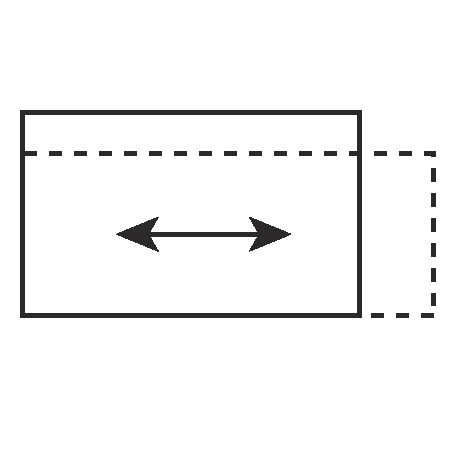
\includegraphics[width=80mm]{images/uniform_strain.pdf}
\caption{two-dimensional simple stretch problem}
\end{figure}


If pulling in the x direction, no force acts in the y direction, so the vertical stress in the y direction becomes 0.

\begin{eqnarray}
\sigma_{yy}=0
\end{eqnarray}



\subsubsection{planar distortion problem}

\begin{equation}
\sigma_{yy}=\lambda\epsilon_{xx}+(\lambda+2\mu)\epsilon_{yy}+\lambda\epsilon_{zz}=\lambda\epsilon_{xx}+(\lambda+2\mu)\epsilon_{yy}=0
\end{equation}


Than,
\begin{equation}
\epsilon_{yy}=-\frac{\lambda}{\lambda+2\mu}\epsilon_{xx}
\end{equation}

.

\begin{equation}
\nu^*=-\frac{\epsilon_{yy}}{\epsilon_{xx}}=\frac{\lambda}{\lambda+2\mu}=\frac{\nu}{1-\nu}
\end{equation}

.


$\sigma_{xx}=(\lambda+2\mu)\epsilon_{xx}+\lambda\epsilon_{yy}=(\lambda+2\mu)\epsilon_{xx}+\lambda(-\frac{\lambda}{\lambda+2\mu})\epsilon_{xx}=\frac{4\mu(\lambda+\mu)}{\lambda+2\mu}\epsilon_{xx}$


From now on, the apparent Young's modulus $E^*$



\begin{equation}
E^*=\frac{\sigma_{xx}}{\epsilon_{xx}}=\frac{4\mu(\lambda+\mu)}{\lambda+2\mu}=\frac{E}{1-\nu^2}
\end{equation}




\subsubsection{plane stress state}


In the planar stress state, it is $\sigma_{zz}=0$, which is consistent with the three-dimensional simple tension. Accordingly

\begin{equation}
\nu^*=\nu,\;\;\;E^*=E
\end{equation}

.



\section{4 points to be aware of when analyzing linear elastic body}


Careful attention to the analysis of the linear elastic body is as follows as four points.

\begin{enumerate}
\item Accuracy of solution drops as Poisson's ratio approaches 0.5.
\item The bending problem is bad in the accuracy of the solution depending on the type of the element
\item Deformation, distortion, stress are evaluated smaller than actual.
\item In the problem of object rotation, the mesh expands and gets unrealistic solution.
\end{enumerate}

Each of the following points will be briefly described below.

\subsection{About the problem that the accuracy of solution decreases when Poisson's ratio approaches 0.5}


As the Poisson's ratio approaches 0.5, the bulk modulus increases infinitely.
This means that the reaction force against volume change becomes large,
An incompressible constraint condition that there is no volume change is gradually added to the displacement.

In the case of such an uncompressed problem, stress is generated by a non-determinate stress generated from a constraint force in addition to the stress generated from the displacement, so it is not possible to analyze only displacement as a variable. We analyze this problem by introducing pressure variables. Analysis of elastic bodies using displacement variables and pressure variables is called u / p formulation. Adding pressure nodes to introduce pressure variables, but since the analysis has good patterns in the manner of placement within the elements of pressure nodes and displacement nodes, they must be adopted.


\subsection{About bending problems depending on the type of elements for problems with poor solution accuracy}


When analyzing the bending of a thin structure such as a beam when the degree of the interpolation function such as the primary element is low,
Solutions that are harder than actual are obtained.
This is a phenomenon called membrane locking and attention is necessary.

This also adds to the displacement the Kirchhoff condition that the out-of-plane shear is 0 when bending a thin structure like a beam, so the accuracy of the solution deteriorates.

High accuracy can be improved by using higher order elements, using reduced integration and selective reduced integration.
It is also effective to stop the solid element and use structural elements.

The details of the rocking problem of the two-dimensional beam bending problem are detailed below.
: Study on Accuracy of 2D Elastic Body Element in Finite Element Method | http: //globe.nagaokaut.ac.jp/yoshisyu/2003/kensetu/pdf/ken04607.pdf

\subsection{About the problem that deformation, distortion, and stress are evaluated to be smaller than actual}


From the variational principle, the analytical solution is the solution with the lowest potential energy. The solution obtained by the finite element method is limited to a function that can be expressed on the mesh, and it is the solution with the smallest energy among them. Therefore, the energy of the finite element method is always larger than the energy of the analytical solution. Roughly speaking, this means that the deformation, strain and stress of the finite element method are evaluated smaller than the deformation of the analytical solution. One purpose of the elastic body analysis by the finite element method is whether or not the structural member breaks. It is evaluated as harder to break than actual. This is dangerous. Careful attention must be paid, such as analyzing different mesh sizes and seeing convergence.

\subsection{The problem of rotating the object about the problem that the mesh expands to obtain an unrealistic solution}


Since the constituent formula of the linear elastic body does not satisfy the objectivity, it is unexpected to rotate.
When the linear elastic body is rotated, an expansion solution is obtained.

The figure below shows the cantilever of a linear elastic body bent under a downward gravity force. It turns out that the rotated part expands greatly and is unrealistic deformation.

\begin{figure}[hptb]
\begin{center}
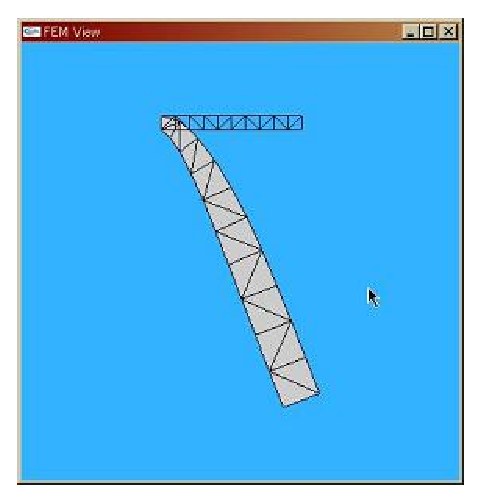
\includegraphics[width=5cm]{images/l_beam.eps}
\end{center}
\caption{inflation if the linear solid material when it is rotated}
\end{figure}

First of all, linear elastic bodies should only be used for micro deformation micro distortion problem. The St. Venant-Kirchhoff body is also compatible with large deformation (that is rotation) due to micro distortion problem.

\subsubsection{detailed analysis of rotation of linear elastic body}


Let's examine in detail what happens when a two-dimensional linear elastic body is rotated in a rigid body.

The coordinate $(x,y)$ in the case where the point $(X,Y)$ is rotated by the $\theta$ rigid body counterclockwise around the origin,

$(x,y)=(X\cos\theta-Y\sin\theta,X\sin\theta+Y\cos\theta)$

The displacement $u_x,u_y$ from the point before rotation

$(u_x,u_y)=(x-X,y-Y)=(X(\cos\theta-1)-Y\sin\theta,X\sin\theta+Y(\cos\theta-1))$

Therefore, the linear distortion becomes as follows.

\begin{eqnarray}
\epsilon_{xx} &=& \frac{\partial u_x}{\partial X}=\cos\theta-1\\
\epsilon_{yy} &=& \frac{\partial u_y}{\partial Y}=\cos\theta-1\\
\gamma_{xy}  &=& \frac{\partial u_x}{\partial Y}+\frac{\partial u_y}{\partial X}=0
\end{eqnarray}


Therefore, it can be seen that vertical distortion of isotropic compression is generated from $\epsilon_{xx}=\epsilon_{yy}<0$. Stress acting to expand by vertically compressing works. Since no stress is applied to the rotating part of the beam, in order to make the stress zero, eventually, an expanded solution is obtained.


\section{Mathematical topics}


Define the norm as follows

\begin{equation}
||\epsilon(v)||^2_0=\int_{\Omega}\epsilon(v):\epsilon(v)d\Omega
\end{equation}

\begin{equation}
||v||^2_0=\sum_{i=1}^N \int_\Omega v_i^2 d\Omega
\end{equation}

\begin{equation}
||v||^2_1=||v||^2_0+\sum_{i=1}^N||\nabla v_i||^2_0
\end{equation}


The weakly shaped linear elastic body is as follows
\begin{equation}
\int_{\Omega} A \epsilon(u):e(\phi)d\Omega = <f,\phi>_{H^{-1},H^1(\Omega)^N}\qquad\qquad\forall\phi\in H^1_\Gamma(\Omega)^N
\end{equation}


Here, substitute $u$ for $\phi$, and from $A$'s stubbornness
\begin{equation}
\alpha||\epsilon(u)||^2_0\le\int_{\Omega} A \epsilon(u):\epsilon(u)d\Omega = <f,u>_{H^{-1},H^1(\Omega)^N} \le ||f||_{H^{-1}} ||u||_1
\end{equation}


\subsection{uniqueness of solution existence}


Korn's first inequality holds.

\begin{equation}
c||v||^2_1\le ||v||^2_0+||\epsilon(v)||^2_0\qquad\qquad\forall v\in H^1(\Omega)^N
\end{equation}


\subsubsection{Korn's second inequality}


Korn's second inequality

\begin{equation}
c'||v||^2_1\le ||\epsilon(v)||^2_0\qquad\qquad\forall v\in H^1_{\Gamma}(\Omega)^N
\end{equation}


It shows by backhoe method that it holds. If the top does not hold,

Fulfilling $||v_n||_1 = 1$

$v_n$ like $\lim_{n\rightarrow \infty}||\epsilon(v_n)||_0=0$ exists. Assuming this, it indicates that contradiction occurs.

From the reserve theorem of Sovlev $H^1$ space is compact in $L^2$ space. Therefore,
\begin{equation}
v_n \rightarrow v \;\;strongly\;in\;\; L^2(\Omega)^N
\end{equation}


There is such $v\in H^1_\Gamma(\Omega)^N$.

Here, from Korn's inequality

\begin{equation}
c||v_n-v_m||^2_1\le ||v_n-v_m||^2_0+||\epsilon(v_n-v_m)||^2_0\\\le ||v_n-v_m||^2_0+||\epsilon(v_n)||^2_0+||\epsilon(v_m)||^2_0
\end{equation}


If you increase $n,m$ you can make the right side as small as you want. Thus $v_n$ is a Cauchy string on $H^1(\Omega)^N$. Therefore $v_n$ converges to $v$ with $H^1(\Omega)^N$.

\begin{equation}
||\epsilon(v)||_0=\lim_{n\rightarrow \infty}||\epsilon(v_n)||_0=0
\end{equation}

Because it is $\epsilon(v)=0$.

Since $v$ is 0 on the boundary $\Gamma$, it is $v=0$.

This is contrary to $||v_n||_1 = 1$. So the title was shown.


\subsubsection{Equality of norm of zzzokljsd with strain tensor and displacement}



Since the inverse inequality is self explanatory, it can be said that $||\phi||_1$ and $||\epsilon(\phi)||_0$ are equivalent norms.

That is, the ellipticity in the $H^1$ of the operator can be said as follows.

\begin{equation}
\alpha ||u||^2_1 \le \int_{\Omega} A \epsilon(u):\epsilon(u)d\Omega\le C ||u||^2_1
\end{equation}


From this, it can be said that there is only solution $u\in H^1_\Gamma(\Omega)^N$ from Lax-Milgram's theorem.




%\section{What I referred to}

%\ cite {Braess 200704}, \ cite {197902}, \ cite {nabe_lecture}, \ cite {hisada 19909}, \ cite {solid_master}, \ cite {chadwick_ 197902}

%\ bibliographystyle {tipsj}
%\ bibliography {.. / main}

\end{document}
